\documentclass{report}
\usepackage[pdftitle={AXI Master and Slave demo},colorlinks=true,urlcolor=blue,breaklinks=true]{hyperref}
\usepackage[edges]{forest}
\usepackage{register}
\usepackage{graphicx}
\title{AXI Master and Slave demo}
\author{Christopher R. Bowman}
\date{3 May 2025}
\begin{document}
\maketitle
\tableofcontents
\listoffigures
\listoftables
\pagebreak
\pagestyle{headings}
\chapter{Introduction}
This project implements the most basic AXI Master interface controlled by a
AXI lite slave register set.  One register controls the read address for the
master.  Another triggers a read by the master from main memory which value
is stored in yet another register that can be read from the slave register
set.
A git repository is located on
\href{https://github.com/}
{github}.
The project is targeted at the AMD/Xilinx Vivado 2024.2 Design Suite.

\chapter{Licensing}
All materials in the repository are Copyright \copyright\ 2025 by
Christopher R. Bowman and all rights are reserved.

Under no circumstances should anything be committed to the
project repository containing copyrighted material which is
owned by a third party.

At some point this project may move to a more permissive licenses.
At present, however, all contributions will have to either donate
the code and copyright or include a world wide, unrestricted
license including the right to create and distribute derivitive
works and sublicense the orignal and derivitive works.

\chapter{Required Software}
AMD/Xilinx Vivado 2024.2 Design Suite

Linux (Rocky 9.4)

FreeBSD (Drivers are QAed for 14.2)

GNU Make

git

wget

fetch

Latex

dvips

dvipdf

latex register packge

\chapter{Repository File Organization}

\definecolor{folderbg}{RGB}{124,166,198}
\definecolor{folderborder}{RGB}{110,144,169}
\newlength\Size
\setlength\Size{4pt}
\tikzset{%
  folder/.pic={%
    \filldraw [draw=folderborder, top color=folderbg!50, bottom color=folderbg] (-1.05*\Size,0.2\Size+5pt) rectangle ++(.75*\Size,-0.2\Size-5pt);
    \filldraw [draw=folderborder, top color=folderbg!50, bottom color=folderbg] (-1.15*\Size,-\Size) rectangle (1.15*\Size,\Size);
  },
  file/.pic={%
    \filldraw [draw=folderborder, top color=folderbg!5, bottom color=folderbg!10] (-\Size,.4*\Size+5pt) coordinate (a) |- (\Size,-1.2*\Size) coordinate (b) -- ++(0,1.6*\Size) coordinate (c) -- ++(-5pt,5pt) coordinate (d) -- cycle (d) |- (c) ;
  },
}
\forestset{%
  declare autowrapped toks={pic me}{},
  pic dir tree/.style={%
    for tree={%
      folder,
      font=\ttfamily,
      grow'=0,
    },
    before typesetting nodes={%
      for tree={%
        edge label+/.option={pic me},
      },
    },
  },
  pic me set/.code n args=2{%
    \forestset{%
      #1/.style={%
        inner xsep=2\Size,
        pic me={pic {#2}},
      }
    }
  },
  pic me set={directory}{folder},
  pic me set={file}{file},
}

\begin{forest}
  pic dir tree,
  where level=0{}{% folder icons by default; override using file for file icons
    directory,
  },
    [axi\_master\_and\_slave
    	[README.md,file]
    	[LICENSE,file]
    	[Makefile,file]
    	[documentation
    		[Makefile,file]
    		[specification.tex,file]
    	]
    	[hardware]
    	[software]
    ]
\end{forest}

\begin{forest}
  pic dir tree,
  where level=0{}{% folder icons by default; override using file for file icons
    directory,
  },
	[hardware
		[GNUmakefile,file]
		[scripts
			[ps7prop\_dict.tcl,file]
			[project.tcl,file]
		]
		[source
			[verilog
				[AXI\_master\_and\_slave.v,file]
				[AXI\_slave.v,file]
				[AXI\_master.v,file]
			]
			[constraints
				[Arty-Z7-20-Master.xdc,file]
			]
		]
	   [verification
            [AXI\_master\_and\_slave\_bd\_wrapper]
	   ]
	]
\end{forest}

\begin{forest}
  pic dir tree,
  where level=0{}{% folder icons by default; override using file for file icons
    directory,
  },
	[software
		[app]
		[driver
			[freebsd
			[Makefile,file]
				[kld
					[README,file]
					[Makefile,file]
					[zynq-artyz7.dtb,file]
					[AXI\_master\_and\_slave.c,file]
					[artyz7\_axi\_mas\_overlay.dts,file]
					[zynq-artyz7.dts,file]
					[zynq-7000.dtsi,file]
				]
			]
		]
	]
\end{forest}

\chapter{Board Design}
The board design has Verificaiton IP (VIP) for clock, reset and AXI interfaces.  When building
the board design these VIPs pass through their signals.  In the verification testbench provided
in the verification directory, these VIPs are configured to drive their respective signals and
thus wrap the master slave block allowing it's verification since the processor subsystem
doesn't have a model.
\begin{figure}[h]
	\begin{center}
			\scalebox{0.45}{
				\includegraphics[width=30cm, height=30cm]{board_design.ps}
			}
	\end{center}
\caption{Board design}
\end{figure}

\chapter{Verification}
A basic verification testbench is provided that writes and reads several slave interface
registers.
Clock and reset VIPs are used to provide clock and reset.  The VIP connected to the master
interface implements a memory models such that read of a memory location will return the
results of the most recent write to that location.

\chapter{Resources}
The following paragraphs provide links to important resources of
relevance to this project as most materials are copyrighted and
cannot be distributed or included in the project git repostories.
It is recommended that you visit the links, download the materials
and keep a local copy for your use.

The board used for this project is the 
\href{https://digilent.com/shop/arty-z7-zynq-7000-soc-development-board/}
{Digilent Arty Z7-20}
available from Digilent.  Documentation for this board can be found on the
\href{https://digilent.com/reference/programmable-logic/arty-z7/reference-manual?redirect=1}
{Arty Z7 Reference Manual} web page. 

The \href{https://www.amd.com/en/products/adaptive-socs-and-fpgas/soc/zynq-7000.html}
{AMD/Xilinx Zynq FPGA} contained on the board is documented in a variety
of manuals.  Of particular interest is the
\href{https://docs.xilinx.com/v/u/en-US/ug585-Zynq-7000-TRM}
{Zynq-7000 SoC Technical Reference Manual UG585}.

\chapter{Programming}
Insert the SD card with the image and at the U-Boot prompt enter the following
commands:

\texttt{fatload mmc 0 400000 bit/ssd\_top.bit}

\texttt{fpga loadb 0 400000 \textit{size}}

Alternatively one can run the following command as root:
\texttt{xbit2bin \textit{fpga.bit}} where \texttt{\textit{fpga.bit}} is the
FPGA bitsream file generated by the AMD/Xilinx tools.  You can also program
from within Vivado on a machine connected via the console/programming port.

\chapter{Register Specifcation}
This design has 4, 32-bit registers which identify the hardware and allow control.
The first register has a fixed ID code and always reads back the same fixed value.
Register 1 sets an address for the master to read from and register 2 receives and
stores the value read from the main memory address in register 1.  Register 3 when,
written, causes the master to read from the main memory and store the results in
register 2 which can then be read back.

The regsiter map is shown in
Table~\ref{table:bar0regmap} on page
~\pageref{table:bar0regmap}.  

\begin{table}[h]
\begin{tabular}{||l|l||}
\hline
 0x0000 & IP Identification register\\
\hline
 0x0004 & Master main memory read fetch address \\
\hline
 0x0008 & Main memory read fetch result \\
\hline
 0x000C & Write only register triggering main memory read \\
\hline
\end{tabular}
\caption{Register Map}
\label{table:bar0regmap}
\end{table}



\begin{register}{h}{IP Identification}{0x0000}% name=CONFIG
\label{ID}%
\regfield{ID}{32}{0}{0xFEEDFACE}% STATUS
\reglabel{Reset}\regnewline%
\begin{regdesc}\begin{reglist}[Request~Depth]
\item [ID](Read only) Containts the constant 0xFEEDFACE 
\end{reglist}\end{regdesc}\end{register}

\begin{register}{h}{Right Digit}{0x0004}% name=CONFIG
\label{RD}%
\regfield{RESERVED}{26}{7}{0}%
\regfield{AA}{1}{6}{0}%
\regfield{AB}{1}{5}{0}%
\regfield{AC}{1}{4}{0}%
\regfield{AD}{1}{3}{0}%
\regfield{AE}{1}{2}{0}%
\regfield{AF}{1}{1}{0}%
\regfield{AG}{1}{0}{0}%
\reglabel{Reset}\regnewline%
\begin{regdesc}\begin{reglist}[Request~Depth]
\item [AA]Setting this bit enables the right AA segment
\item [AB]Setting this bit enables the right AB segment
\item [AC]Setting this bit enables the right AC segment
\item [AD]Setting this bit enables the right AD segment
\item [AE]Setting this bit enables the right AE segment
\item [AF]Setting this bit enables the right AF segment
\item [AG]Setting this bit enables the right AG segment
\end{reglist}\end{regdesc}\end{register}

\begin{register}{h}{Left Digit}{0x0008}% name=CONFIG
\label{LD}%
\regfield{RESERVED}{26}{7}{0}%
\regfield{AA}{1}{6}{0}%
\regfield{AB}{1}{5}{0}%
\regfield{AC}{1}{4}{0}%
\regfield{AD}{1}{3}{0}%
\regfield{AE}{1}{2}{0}%
\regfield{AF}{1}{1}{0}%
\regfield{AG}{1}{0}{0}%
\reglabel{Reset}\regnewline%
\begin{regdesc}\begin{reglist}[Request~Depth]
\item [AA]Setting this bit enables the left AA segment
\item [AB]Setting this bit enables the left AB segment
\item [AC]Setting this bit enables the left AC segment
\item [AD]Setting this bit enables the left AD segment
\item [AE]Setting this bit enables the left AE segment
\item [AF]Setting this bit enables the left AF segment
\item [AG]Setting this bit enables the left AG segment
\end{reglist}\end{regdesc}\end{register}


\begin{register}{h}{RESERVED}{0x000C}% name=CONFIG
\label{RES}%
\regfield{RESERVED}{32}{0}{0}%
\reglabel{Reset}\regnewline%
\begin{regdesc}\begin{reglist}[Request~Depth]
\item [RESERVED] (Read only) This registers is reserved and always read as 0x0
\end{reglist}\end{regdesc}\end{register}

\end{document}
